\documentclass[12pt]{article}


\usepackage[dvips,letterpaper,margin=0.75in,bottom=0.75in]{geometry}
\usepackage{cite}
\usepackage{slashed}
\usepackage{graphicx}
\usepackage{amsmath}

\usepackage[american,fulldiode]{circuitikz}

\begin{document}
\ctikzset{bipoles/thickness=1}
\ctikzset{bipoles/length=.6cm}

\title{Introduction to the Arduino and Scientific Python} 

\maketitle

\section{Introduction}

In this lab, we will learn to use the Arduino microprocessor and scientific python, two tools we will be using through out this course.


\section{Introduction to the Arduino}

For this lab, we will use Arduino Uno.  The Arduino Uno is fairly robust and inexpensive, so you should definitely be comfortable to experiment with them.  However, to avoid the potential to damage the boards, you should *NOT* supply any external power to the Arduino (e.g. from your proto-board PB-503, bench-top power supply, or function generator.)  


https://www.arduino.cc/en/Guide/ArduinoUno

\vspace{0.5 cm}

\noindent
{\bf Step 1:} The main Arduino website, which includes lots of
supporting documentation, is located at {\tt http://arduino.cc}.
Acquaint yourself with this site. 
\vspace{0.5 cm}

\noindent
{\bf Step 2:} The lab PCs have the Arduino software installed, and
each team will have an Arduino to work with.  Follow the instructions
for using the ``Arduino Desktop IDE" located here:  
{\tt https://www.arduino.cc/en/Guide/ArduinoUno}.
\vspace{0.5 cm}

\noindent
{\bf Step 3:} Adjust the pattern of the LED blink example to a slower rate. 
\vspace{0.5 cm}

\noindent
{\bf Step 4:}  The Arduino tutorials and built-in-examples are often excellent starting points for you own projects, browse the tutorials here:\\
https://www.arduino.cc/en/Tutorial/HomePage
\vspace{0.5 cm}

\begin{figure}[htbp]
\begin{center}
\begin{circuitikz}[line width=1pt]
\draw(0,0) node[right]{5 V} to[resistor,l_=$R_1$,o-o] ++(0,-2) node[right]{($+$)} to[push button, l=$S_1$,bipoles/length=1.2cm] ++(0,-2) node[ground,yscale=2.0]{};
\end{circuitikz} 
\caption{
On the proto-board shield, the push-button switch S1 shorts the point labeled ``+'' to ground
  when pressed.  Use a pull-up resistor $R_1=10~\rm k\Omega$ to set the voltage at point $+$ to 5~V unless the push-button $S_1$ is engaged.}
\label{fig:pullup}
\end{center}
\end{figure}

\noindent
{\bf Step 5:} Read, build and upload the DigitalReadSerial example.  You will need the Arduino proto-shield, which includes a pushbutton and LEDs, to complete this part. Note: to use the
pushbutton switch labeled S1 on the Prototype Shield v.5, note that hole labeled
(+) is shorted to ground when the push button is pressed.  Your protoboard shield should already have a wire soldered at this point.  Use a pull-up resistor as shown if Fig.~\ref{fig:pullup}.
\vspace{0.5 cm}

\noindent
{\bf Step 6:} Modify it to only output to the serial port after a change in value.
\vspace{0.5 cm}

\noindent
{\bf Step 7:} Read, build and upload the Read Analog Voltage example.  You will need a potentiometer (variable resistor) for this and the following step.
\vspace{0.5 cm}

\noindent
{\bf Step 8:} Read, build, and upload the Analog Input example. \\
\vspace{0.5 cm}

\section{Introduction to Scientific Python}
%{\tt https://www.scipy-lectures.org/\_downloads/ScipyLectures-simple.pdf}\\


Much of our work will be using scientific python in an interactive notebook environment.  On some of the newer lab PCs, this is called ``Jupyter Notebook" while on some of the older PCs, this is installed under it's older name as ``IPython Notebook".  Simply find the icon on your Desktop to start the notebook, click it, and start a new notebook.  Most often, we will want inline plots that show up as output in your notebook.  You enable this by using the special command {\tt \%pylab inline} at the start of your notebook, as demonstrated in Fig.~\ref{fig:notebook}.  This command also imports matplotlib and numpy as ``plt" and ``np" so you will be able to work through the tutorial here:\\
{\tt https://matplotlib.org/users/pyplot\_tutorial.html}\\
by simply omitting the ``import" directives from the example code snippets.
\begin{figure}[htbp]
\begin{center}
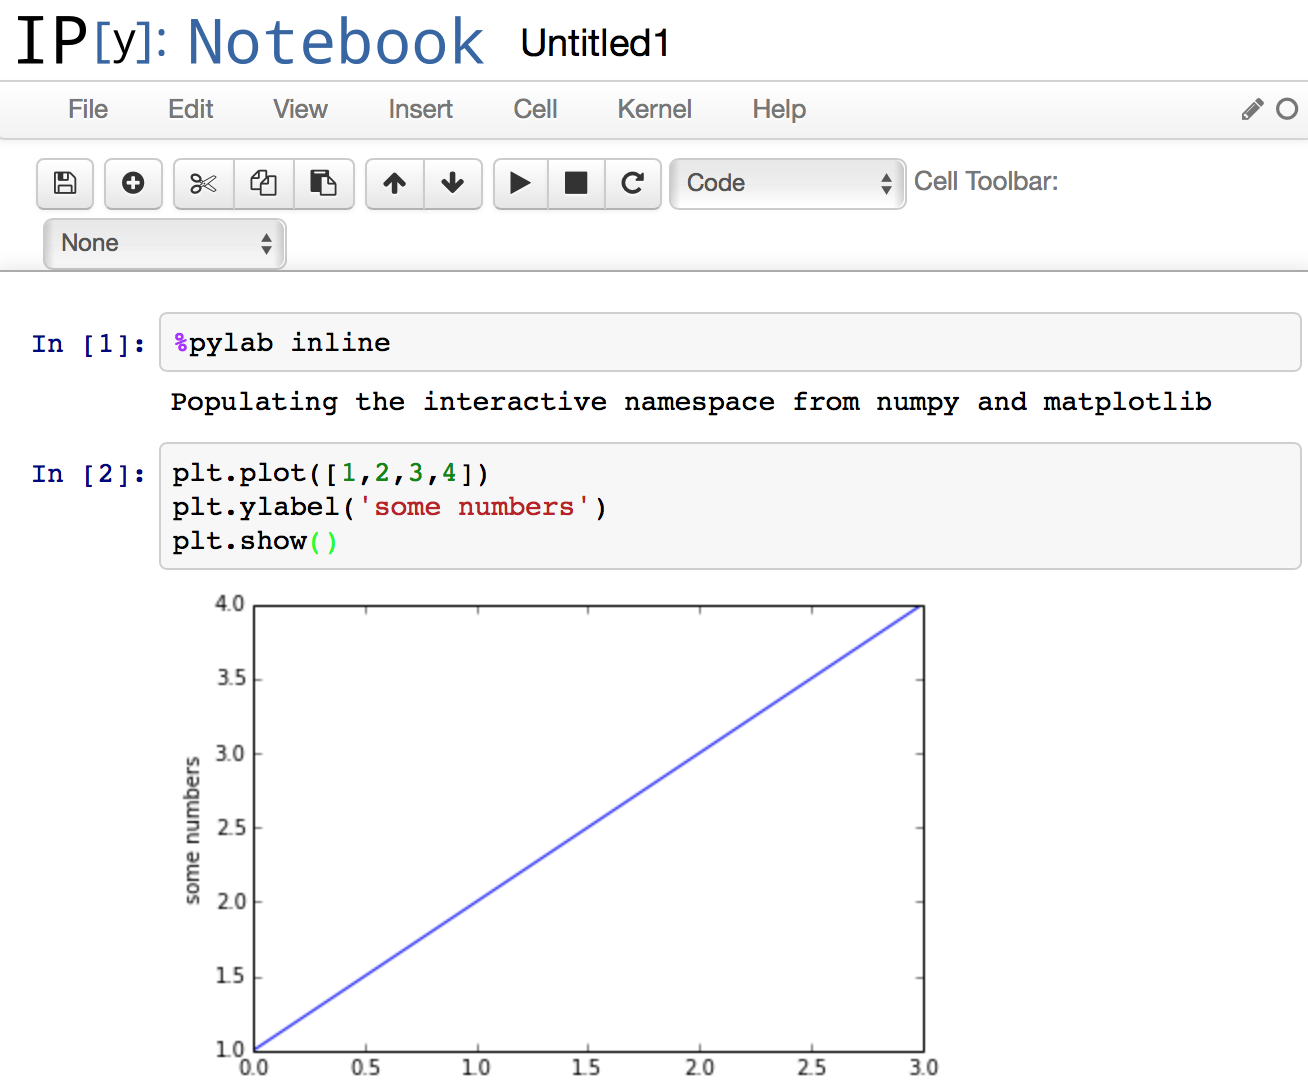
\includegraphics[width=0.95\textwidth]{figs/notebook.png}\\
\caption{\label{fig:notebook}
Using Jupyter notebook in inline mode to start the Matplotlib tutorial.}
\end{center}
\end{figure}
Note that some of the code snippets are not complete examples.  You should only try to run the complete examples which include the expected output and begin with an ``import" command (which you will omit.)  Also, note that our installation does not include the {\tt logit} scale, so simply replace {\tt logit} with {\tt log} for the last example.   See Fig.~\ref{fig:notebook} to get started.

\section{Lab Report}

There is no lab report for this lab, simply inform your TA when you have completed everything.
 
\end{document}
